\documentclass[a4paper,12pt]{article}
\usepackage{amsmath}
\usepackage{graphicx}
\usepackage{enumitem}
\usepackage{booktabs}
\usepackage{listings}
\usepackage{hyperref}
\usepackage{tikz}

\title{Trade-offs in FRF Measurements}
\author{}
\date{}
\begin{document}

% Cover page information
\begin{center}
    \Large \textbf{Measurement and Data Driven Modeling}\\
    \vspace{0.3cm}
    \LARGE \textbf{Assignment Report}\\
    \vspace{0.5cm}
    \Large \textbf{Trade-offs in FRF Measurements}\\
    \vspace{1cm}
\end{center}

\section*{Objective}
This assignment aims to explore and demonstrate the practical trade-offs between:
\begin{enumerate}
    \item Frequency resolution
    \item Measurement time
    \item Signal-to-Noise Ratio (SNR)
\end{enumerate}
in the context of measuring Frequency Response Functions (FRFs). This understanding is crucial when designing excitation signals for system identification.

\section*{Background}
Measuring accurate FRFs requires balancing three competing factors:
\begin{enumerate}
    \item \textbf{Frequency Resolution}: Higher resolution allows more frequency lines to be distinguished within a given bandwidth.
    \item \textbf{Measurement Time}: Longer signals allow more averaging, reducing random noise.
    \item \textbf{SNR}: The clarity with which excited frequency components emerge from the noise floor.
\end{enumerate}
This trade-off is fundamental and unavoidable in any practical measurement setup. The trade-offs explored in this assignment assume:
\begin{itemize}
    \item The RMS amplitude of the excitation signal is fixed to \(1 \,V\).
    \item The frequency band of interest lies between 5 Hz and 10 Hz.
\end{itemize}

\section*{Multisine Design Summary}
The table below summarizes six example multisines designed to illustrate the trade-offs under different constraints:

\begin{table}[h!]
\centering
\caption{Example Multisine Designs for Each Trade-off Case}
\begin{tabular}{@{}lccc@{}}
\toprule
\textbf{Trade-off Case} & \textbf{Excited Frequencies (Hz)} & \textbf{Period (s)} & \textbf{Notes} \\ \midrule
Fixed Resolution 1 & 5 to 10 Hz (30 lines) & 6 s & Balanced power \\
Fixed Resolution 2 & 5 to 10 Hz (30 lines) & 12 s & Higher SNR \\
Fixed Time 1 & 5 to 10 Hz (30 lines) & 6 s & Baseline \\
Fixed Time 2 & 5 to 10 Hz (60 lines) & 6 s & Finer resolution \\
Fixed SNR 1 & 5 to 10 Hz (30 lines) & 6 s & Target SNR 40 dB \\
Fixed SNR 2 & 5 to 10 Hz (60 lines) & 12 s & Same SNR, more lines \\
\bottomrule
\end{tabular}
\end{table}

\section*{Results and Explanation}

\begin{figure}[h!]
    \centering
    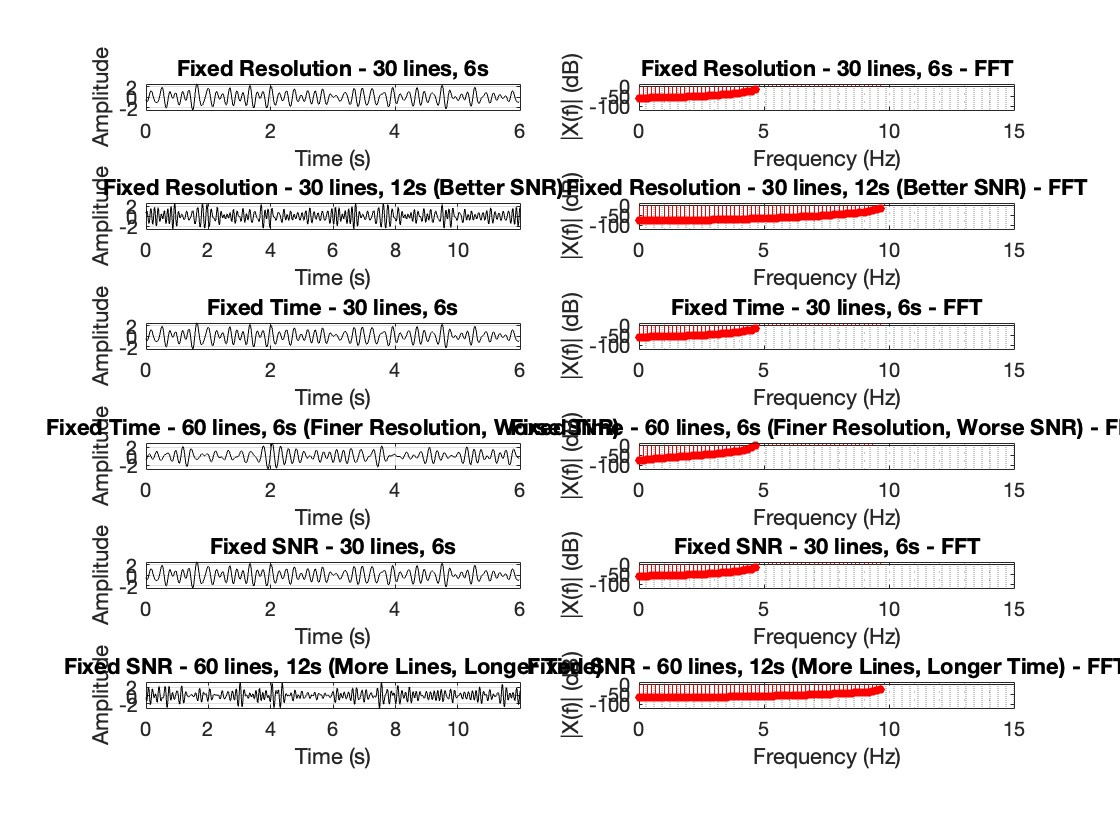
\includegraphics[width=0.9\textwidth]{frftradeoff.jpg}
    \caption{Time and Frequency Domain Plots for Different Multisine Designs Illustrating Trade-offs}
    \label{fig:frf_tradeoff}
\end{figure}

\subsection*{Overview}
Figure \ref{fig:frf_tradeoff} displays the time domain and frequency domain representations of all six multisines. The left column shows the time-domain signals, while the right column shows the corresponding magnitudes of the Discrete Fourier Transform (DFT).

\subsection*{Analysis of Trade-offs}

\subsubsection*{Trade-off 1: Fixed Frequency Resolution}
The first two rows represent cases where 30 equally spaced frequencies between 5 Hz and 10 Hz are excited.
\begin{itemize}
    \item Row 1 uses a 6-second signal.
    \item Row 2 uses a 12-second signal.
\end{itemize}
The longer duration reduces noise variance, improving the SNR. This can be seen from the cleaner peaks in the frequency spectrum of Row 2 compared to Row 1.

\textbf{Physical Reason:} 
A longer time window improves frequency resolution by creating narrower frequency bins, making it easier to distinguish closely spaced frequencies. It also enhances SNR by allowing more averaging, which reduces noise variation and makes signal peaks clearer. This leads to a more accurate and detailed frequency spectrum.

Trade-off: Higher SNR → Longer measurement time, Shorter measurement time → Lower SNR.

\subsubsection*{Trade-off 2: Fixed Measurement Time}
The third and fourth rows correspond to a fixed 6-second measurement duration.
\begin{itemize}
    \item Row 3 excites 30 frequencies.
    \item Row 4 excites 60 frequencies, doubling the resolution.
\end{itemize}
Since the total power (RMS fixed to 1V) must be spread over more frequencies in Row 4, the SNR per frequency decreases. This leads to less distinct peaks in the frequency domain.

\textbf{Physical Reason:} 
The fixed measurement time limits the total energy available in the excitation signal. As more frequency lines are excited (increased resolution), the available power per frequency component decreases. As a result, the peaks in the frequency spectrum become less pronounced relative to noise, this reduces the effective SNR per frequency line. This is a direct consequence of energy spreading across more frequencies. 

Trade-off: Higher FR → Lower SNR, Lower FR → Higher SNR.

\subsubsection*{Trade-off 3: Fixed SNR}
The fifth and sixth rows maintain a constant SNR.
\begin{itemize}
    \item Row 5 excites 30 frequencies over 6 seconds.
    \item Row 6 excites 60 frequencies, requiring the measurement duration to increase to 12 seconds to maintain SNR.
\end{itemize}
This illustrates that improving resolution (more lines) requires a proportional increase in measurement time to maintain SNR.
\\
\\
\textbf{Physical Reason:} 
If more frequencies are excited while keeping SNR constant, the measurement must last longer to allow enough noise averaging. This ensures each frequency gets sufficient energy and remains distinguishable from noise. Higher resolution needs longer measurement time for the same noise suppression.

Trade-off: Higher FR → Longer measurement time, Shorter measurement time → Lower FR.
\subsection*{Summary of Observations}
The experiments confirm the core trade-off triangle:

\begin{center}
    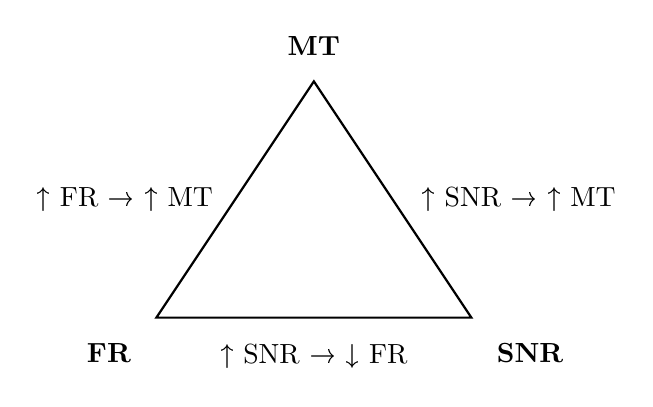
\begin{tikzpicture}
        % Draw the triangle
        \draw[thick] (0,2) -- (-2,-1) -- (2,-1) -- cycle;
        
        % Add labels at each vertex
        \node[above] at (0,2.2) {\textbf{MT}};
        \node[below left] at (-2.2,-1.2) {\textbf{FR}};
        \node[below right] at (2.2,-1.2) {\textbf{SNR}};
        \node at (0,-1.5) {↑ SNR → ↓ FR};
        \node at (-2.4,0.5) {↑ FR → ↑ MT};
        \node at (2.6,0.5) {↑ SNR → ↑ MT};
    \end{tikzpicture}
\end{center}


\begin{itemize}
    \item Increasing measurement time improves SNR at constant resolution.
    \item Increasing resolution reduces SNR if time is fixed.
    \item Maintaining SNR while increasing resolution requires longer measurement times.
\end{itemize}
This triangular trade-off directly reflects the physics of spectral analysis and how energy spreads across time and frequency when the signal RMS is fixed.

\subsection*{Conclusion}
Understanding these physical mechanisms is essential for practical FRF measurements. We must carefully select the combination of resolution, time, and SNR to match the goals of a specific system identification experiment. This trade-off framework applies to many real-world scenarios, such as vibration testing, acoustic analysis, and electromagnetic characterization.
\section*{MATLAB Code Implementation}
The MATLAB code used to generate these results is included below:

\lstset{language=Matlab, basicstyle=\ttfamily\small, breaklines=true}
\begin{lstlisting}
% Trade-offs in FRF Measurement
clc; clear; close all;

% Global parameters
fs = 100;            % Sampling frequency (Hz)
RMS_des = 1;         % Desired RMS value
f_start = 5;         % Start frequency (Hz)
f_end = 10;          % End frequency (Hz)

% Tradeoff 1: Fixed Frequency Resolution
% Multisine 1 - 30 lines, 6 seconds
N1 = fs * 6;                          % 6 seconds worth of samples
frequencies1 = linspace(f_start, f_end, 30);
x1 = generate_multisine(N1, frequencies1, fs, RMS_des);

% Multisine 2 - 30 lines, 12 seconds (better SNR)
N2 = fs * 12;                         % 12 seconds worth of samples
x2 = generate_multisine(N2, frequencies1, fs, RMS_des);

% Tradeoff 2: Fixed Measurement Time
% Multisine 3 - 30 lines, 6 seconds
x3 = x1;  % Same as Multisine 1 (fixed time = same N)

% Multisine 4 - 60 lines, 6 seconds (worse SNR, finer resolution)
frequencies4 = linspace(f_start, f_end, 60);
x4 = generate_multisine(N1, frequencies4, fs, RMS_des);

% Tradeoff 3: Fixed SNR
% Multisine 5 - 30 lines, 6 seconds, fixed SNR
x5 = x1;  % Same as Multisine 1 (same power spread over 30 lines)

% Multisine 6 - 60 lines, 12 seconds (more frequencies, but maintain SNR by longer time)
x6 = generate_multisine(N2, frequencies4, fs, RMS_des);

% Plot all results 
multisines = {x1, x2, x3, x4, x5, x6};
titles = {
    "Fixed Resolution - 30 lines, 6s', ...
    "Fixed Resolution - 30 lines, 12s (Better SNR)', ...
    "Fixed Time - 30 lines, 6s', ...
    "Fixed Time - 60 lines, 6s (Finer Resolution, Worse SNR)', ...
    "Fixed SNR - 30 lines, 6s', ...
    "Fixed SNR - 60 lines, 12s (More Lines, Longer Time)'
};

figure;
for i = 1:6
    subplot(6, 2, 2*i-1);
    plot((0:length(multisines{i})-1)/fs, multisines{i});
    xlabel('Time (s)');
    ylabel('Amplitude');
    title(titles{i});

    subplot(6, 2, 2*i);
    X = fft(multisines{i});
    f = (0:length(X)-1) * (fs/length(X));
    stem(f, abs(X), 'b', 'filled');
    xlabel('Frequency (Hz)');
    ylabel('|X(f)|');
end

disp('All multisines generated and plotted successfully.');

%
function x = generate_multisine(N, frequencies, fs, RMS_des)
    t = (0:N-1) / fs;  % Time vector
    x = zeros(1, N);   % Initialize signal

    for f = frequencies
        phase = 2 * pi * rand();  % Random phase for each frequency
        x = x + cos(2*pi*f*t + phase);
    end

    % Scale to desired RMS
    RMS_x = sqrt(mean(x.^2));
    x = x * (RMS_des / RMS_x);
end

\end{lstlisting}
\end{document}